%!TEX root = ../main.tex

In this section, we utilize the string constraint in Equation~(\ref{eqn-running}) to illustrate the approach in this work.

%$x \in (\Sigma \setminus a)^{\{5, 60\}} (\Sigma \setminus b)^{\{5, 60\}} (\Sigma \setminus c)^{\{0, 60\}} \wedge x \in \Sigma^* c^+ \wedge |x| > 120$.

We first construct an automaton for the regular expression $(\Sigma \setminus a)^{\{5, 60\}} (\Sigma \setminus b)^{\{5, 60\}} (\Sigma \setminus c)^{\{0, 60\}}$. We introduce three registers, say $r_1, r_2, r_3$, to represent the three counting operators.  
%Moreover, we introduce another register, say $r_0$, to denote the length of strings. 
Then we first construct a nondeterministic finite automaton (NFA) for $(\Sigma \setminus a)^* (\Sigma \setminus b)^* (\Sigma \setminus c)^*$, then add the updates of registers to transitions, resulting into a so-called cost-enriched finite automaton (CEFA) $\aut_1$,  as illustrated in Figure~\ref{fig:overview}(a). 
%Then we obtain a cost-enriched finite automaton (CEFA) $\aut_1$ that is illustrated in Figure~\ref{fig:overview}(a), where the self-loops around $p_0, p_1, p_2$ represent the first, second, and third counting operator respectively, in which $r_1, r_2, r_3$ are incremented. 
%Moreover, $r_0$ is incremented in all the three self-loops. 
Furthermore, the counting bounds are specified by the accepting condition $5 \le r_1 \le 60 \wedge 5 \le r_2 \le 60 \wedge 0 \le r_3 \le 60$ that is attached to the final state $p_2$. Note here we represent the counting operators symbolically by registers, instead of unfolding them explicitly. Moreover, we also construct a CEFA $\aut_2$ for $\Sigma^* c^+$ (see Figure~\ref{fig:overview}(b)), which is actually an NFA, since $\Sigma^* c^+$ contains no (explicit) counting operators. 
%where the register $r_0$ is used to record the length of strings. 

% the register $r_1$ is incremented in the two transitions from $q_0$ to $q_0$ and $q_1$ respectively,  the register $r_2$ is incremented in the two transitions from $q_1$ to $q_1$ and $q_2$ respectively, and the register $r_3$ is incremented in the transition from $q_2$ to $q_2$ itself. Moreover, the register $r_4$ is incremented in each transition.  

\begin{figure}[ht]
  \centering
  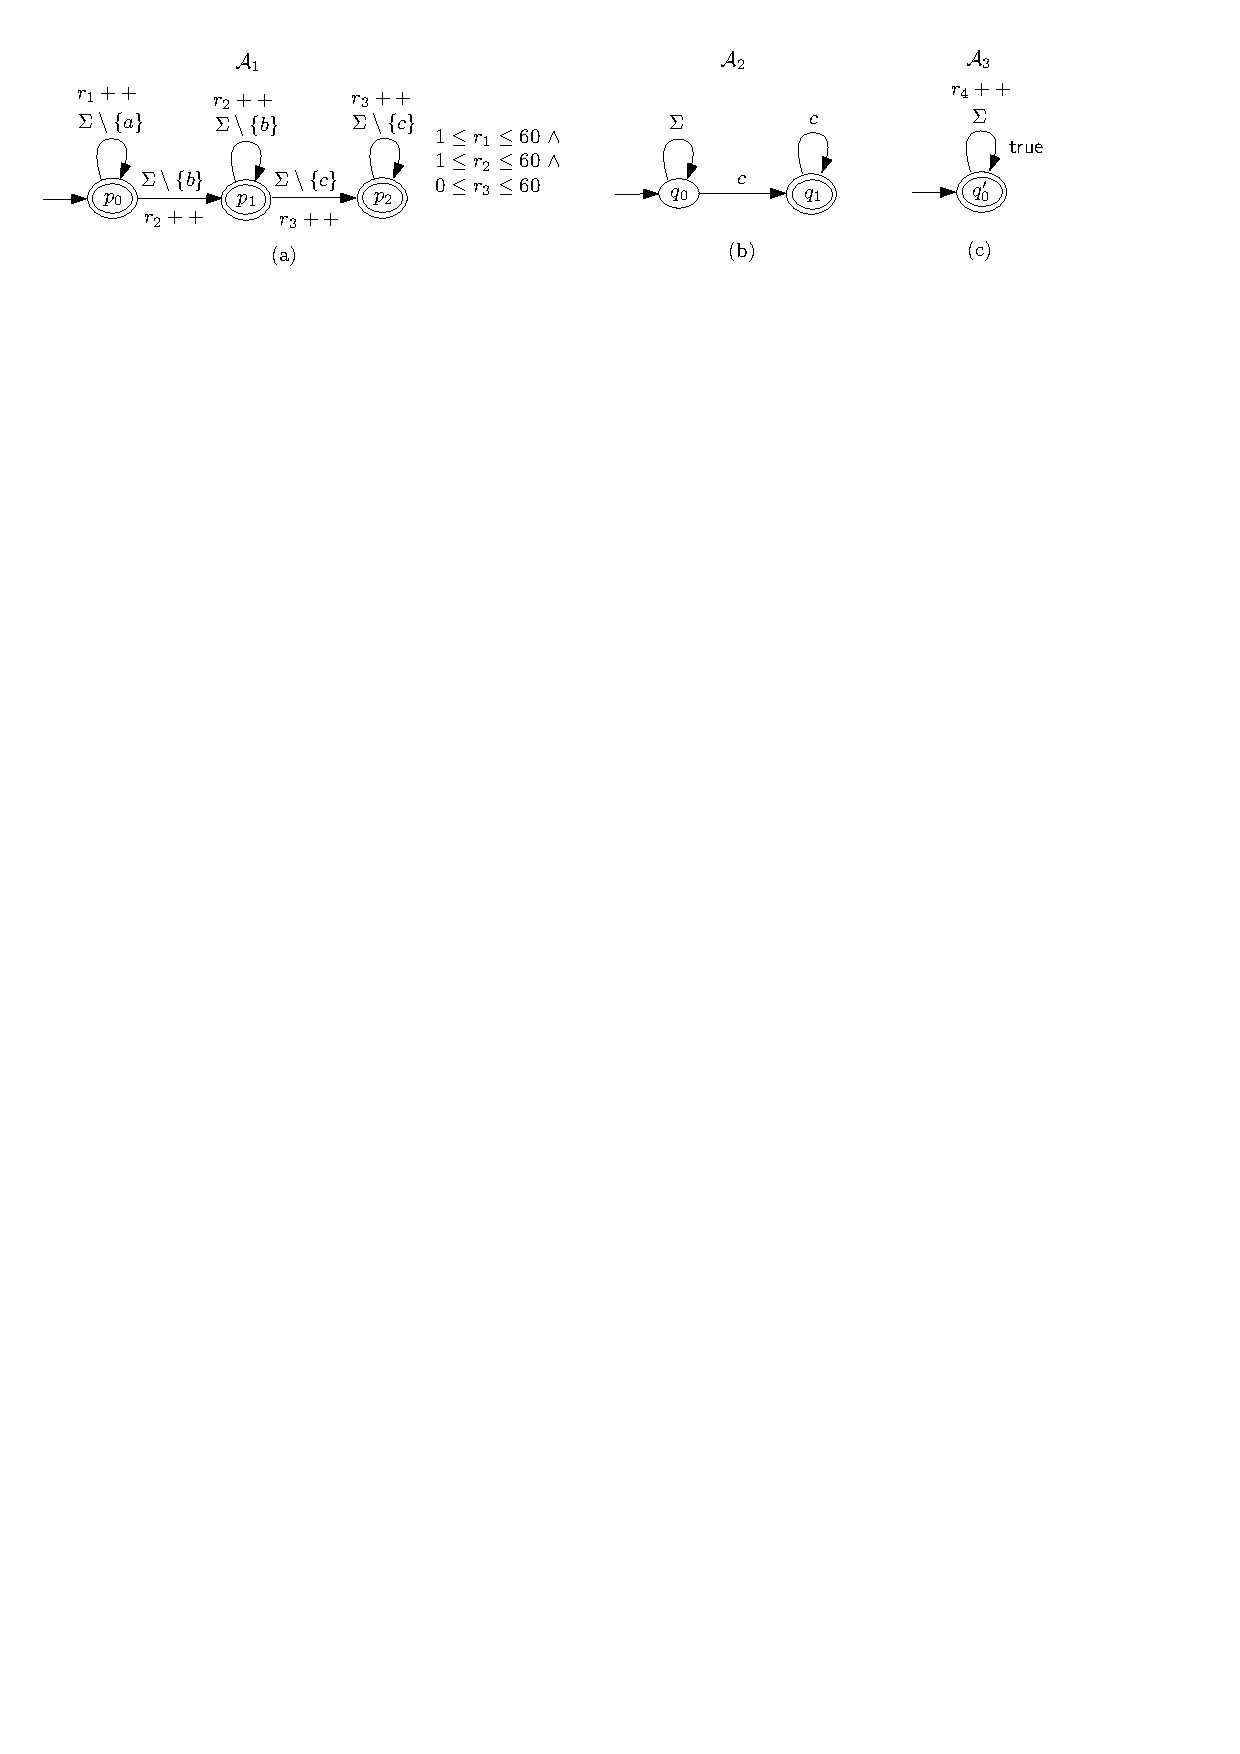
\includegraphics[width = 0.9\textwidth]{sections/overview-cefa.pdf}
  \caption{CEFA for $(\Sigma \setminus a)^{\{5, 60\}} (\Sigma \setminus b)^{\{5, 60\}} (\Sigma \setminus c)^{\{0, 60\}}$ and $\Sigma^* c^+$}
  \label{fig:overview}
\end{figure}

Next, 
%we remove the $\varepsilon$-transitions of $\aut_1$, resulting into $\aut'_1$, 
we construct $\aut_1 \times \aut_2$, that is, the product of $\aut_1$ and $\aut_2$, as illustrated in Figure~\ref{fig:overview:product}(a). Furthermore, we add one special register, say $r_0$, to record the length of strings. Note that $r_0$ is incremented in all transitions. In $\aut_1 \times \aut_2$, the accepting condition $5 \le r_1 \le 60 \wedge 5 \le r_2 \le 60 \wedge 0 \le r_3 \le 60 \wedge r_0 > 120$ is attached to both $(p_0,q_1)$ and $(p_1,q_1)$, where $r_0 > 120$ is added as a conjunct to express $|x| > 120$.  For technical convenience, we also think the updates on the values of registers in transitions as vectors $(v_1, v_2, v_3, v_4)$, where $v_i \in \Int$ is the update on the register $r_{i-1}$ for each $i \in [4]$. For instance, the transitions corresponding to the self-loop around $(p_0, q_0)$ are thought as $(q, a', q', (1,1,0,0))$ with $a' \in \Sigma \setminus \{a\}$, since $r_0$ and $r_1$ are incremented in these transitions. With the updates thought as vectors, the resulting CEFA is illustrated in Figure~\ref{fig:overview:product}(b).
%the transitions corresponding to the self-loop is $(q, a', q', (1,1,0,0))$ with $a' \in \Sigma \setminus \{a\}$.  

\begin{figure}[ht]
  \centering
  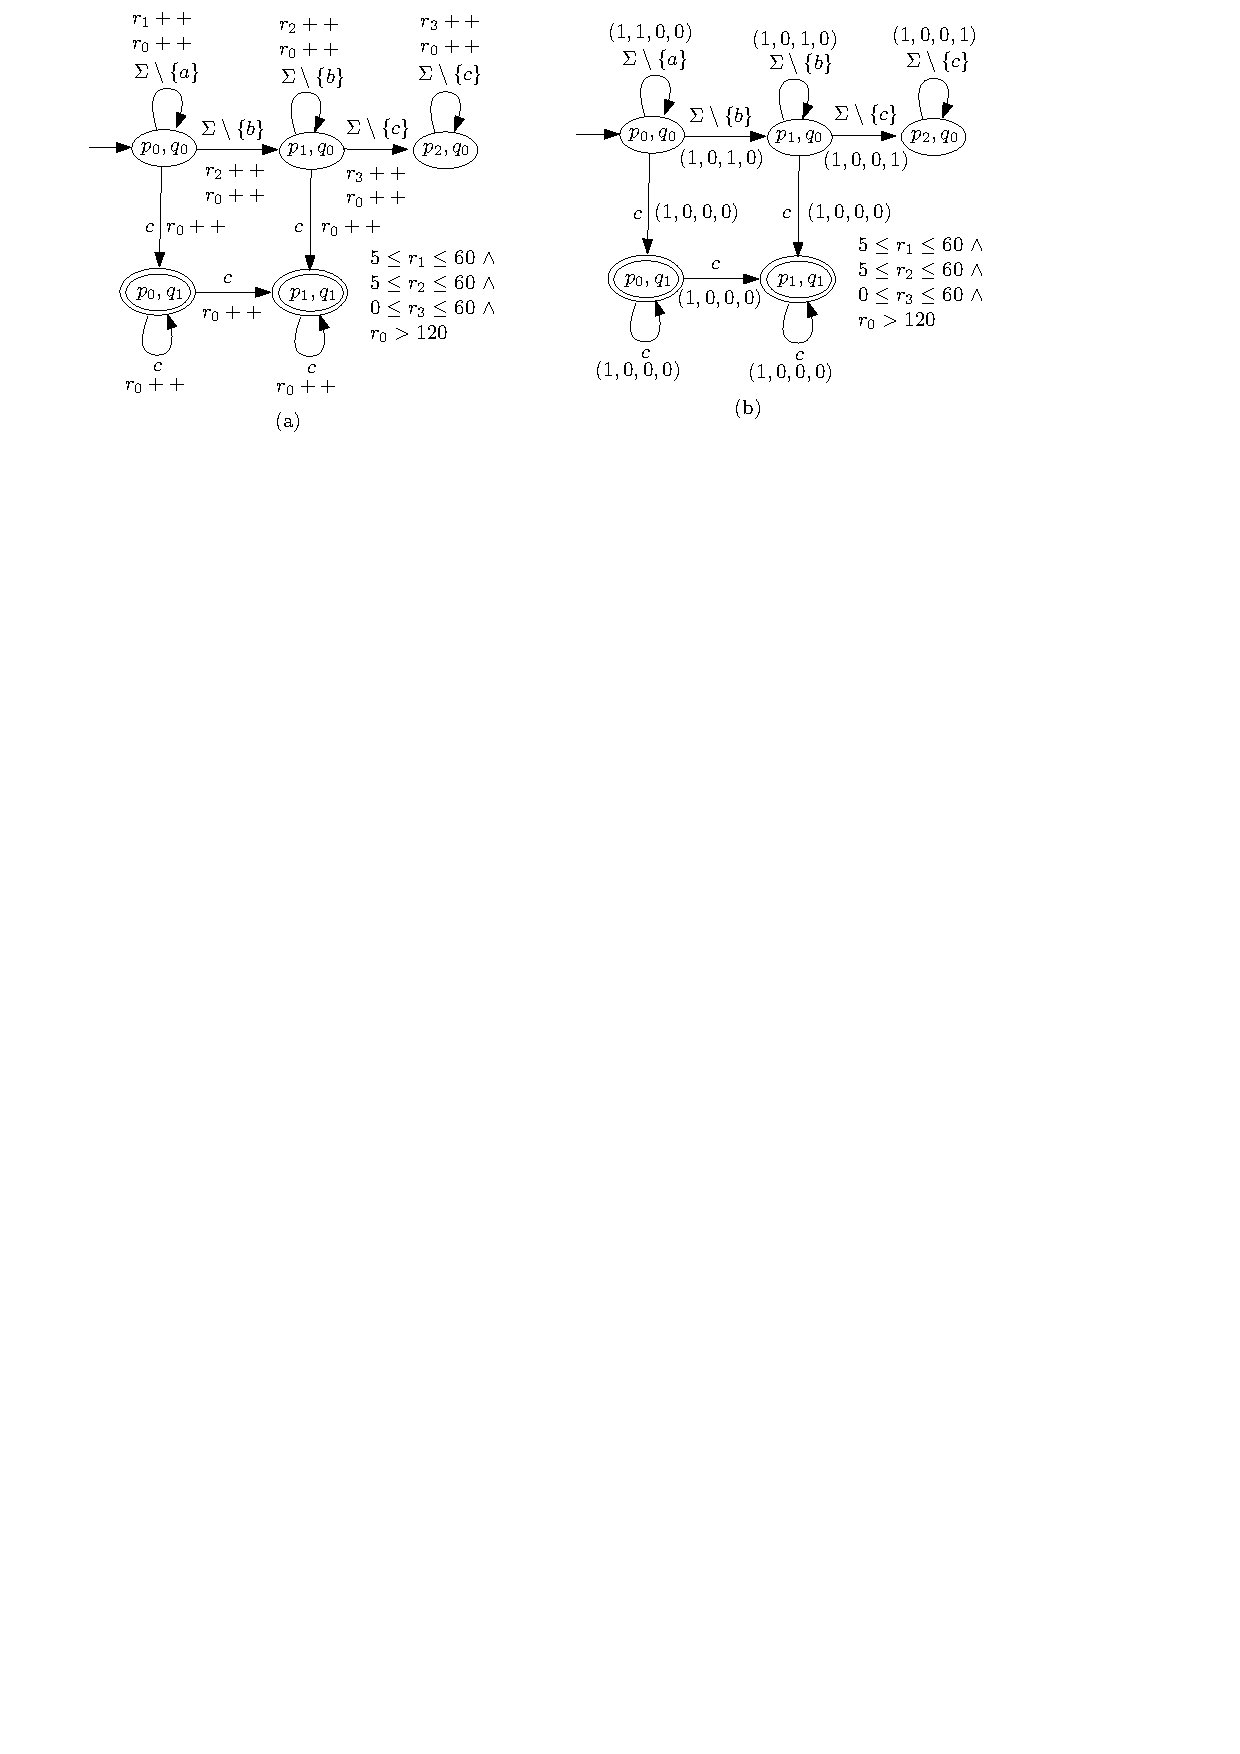
\includegraphics[width = 0.9\textwidth]{sections/overview-cefa-product.pdf}
  \caption{Product of $\aut_1$ and $\aut_2$, where the length register $r_0$ is added}
  \label{fig:overview:product}
\end{figure}

Let $\tau_1, \cdots, \tau_m$ be an enumeration of the transitions of $\aut_1 \times \aut_2$ and $\myvec{v_1}, \cdots, \myvec{v_m}$ be the vectors of updates on the register values in these transitions. For instance, in the transition from $(p_0, q_1)$ to $(p_1, q_1)$, $r_0$ is incremented, and the values of the other registers is unchanged. Therefore, the vector for this transition is $(1, 0, 0, 0)$. 
Then the satisfiability of the original string constraint is reduced to the nonemptiness of the CEFA $\aut_1 \times \aut_2$. 
From the results in \cite{SSMH04,VSS05}, an existential LIA formula $\psi(i_1, \cdots, i_m)$ can be computed to express the constraints on the number of occurrences of $\tau_1, \cdots, \tau_m$ in the accepting runs of $\aut_1 \times \aut_2$, where $i_1, \cdots, i_m$ are the integer variables representing the number of occurrences of $\tau_1, \cdots, \tau_m$ respectively. 
Therefore, the satisfiability of the string constraint in~(\ref{eqn-running}) is reduced to the satisfiability of the following existential LIA formula
\begin{equation}\label{eqn-LIA}
\psi(i_1, \cdots, i_m) \wedge \bigwedge \limits_{0 \le j \le 3} r_j = \sum \limits_{k \in [m]}  i_k v_{k, j+1} \wedge \alpha(r_0, r_1, r_2, r_3),
\end{equation}
where for each $k \in [m]$, $v_k = (v_{k,1}, v_{k,2}, v_{k, 3}, v_{k, 4})$ is the vector of updates on the registers $r_0, r_1, r_2, r_3$ in the transition $\tau_k$, and $\alpha(r_0, r_1, r_2, r_3)$ is the accepting condition in $\aut_1 \times \aut_2$. Finally, the satisfiability of LIA formula can be solved by the off-the-shelf SMT solvers for LIA. 

Nevertheless, since it is well known that the satisfiability of existential LIA formulas is NP-complete (see e.g. \cite{Haase18}), the performance could be improved if the size of the formula in~(\ref{eqn-LIA}) can be reduced. Since the size of the formula in~(\ref{eqn-LIA}) depends on the size of $\aut_1 \times \aut_2$, that is, the number of states, transitions, and registers in $\aut_1 \times \aut_2$, we propose the techniques to reduce the size of the CEFA $\aut_1 \times \aut_2$.

Our main idea to reduce the size of the CEFA $\aut_1 \times \aut_2$ is to \emph{ignore the characters in transitions}, since the updates of the values of registers in transitions are independent of the characters therein and the satisfiability of the formula in~(\ref{eqn-LIA}) only concerns about the values of registers. After the characters in transitions are ignored, each transition in $\aut_1 \times \aut_2$ is of the form $(q, \myvec{v}, q')$, where $\myvec{v}$ is the vector denoting the updates on the values of registers. Let $\cB$ denote the resulting automaton. We then think $\cB$ as an NFA, where the vectors $\myvec{v}$ are taken as the characters. Then we apply the determinization and minimization algorithm of NFAs to $\cB$, resulting into an automaton $\cC$, as illustrated in Figure~\ref{fig:overview:product:reduced}. 
Note that $\cC$ contains only three states $q'_0, q'_1, q'_2$ and six transitions $\tau'_1, \cdots, \tau'_6$, thus containing much less number of transitions than $\aut_1 \times \aut_2$\footnote{This is the case even if we consider subsets of characters, e.g. $\{a\}, \{b\}, \{c\}, \Sigma \setminus \{a, b, c\}$, in the transitions of $\aut_1 \times \aut_2$.}.
Then we reinterpret $\cC$ as a CEFA with the acceptance condition $\alpha(r_0, r_1, r_2, r_3)$. 
Finally, we compute an LIA formula $\psi'(i_1, \cdots, i_6)$ from $\cC$ and reduce the satisfiability of the string constraint in~(\ref{eqn-running}) to the satisfiability of the following existential LIA formula
\begin{equation}\label{eqn-LIA-reduced}
\psi'(i_1, \cdots, i_6) \wedge \bigwedge \limits_{0 \le j \le 3} r_j = \sum \limits_{k \in [6]}  i_k v'_{k, j+1} \wedge \alpha(r_0, r_1, r_2, r_3),
\end{equation}
where $\myvec{v'_{k}}=(v'_{k,1}, v'_{k,2}, v'_{k,3}, v'_{k,4})$ is the vector of updates of registers of the transition $\tau'_k$ for $k \in [6]$.

\begin{figure}[ht]
  \centering
  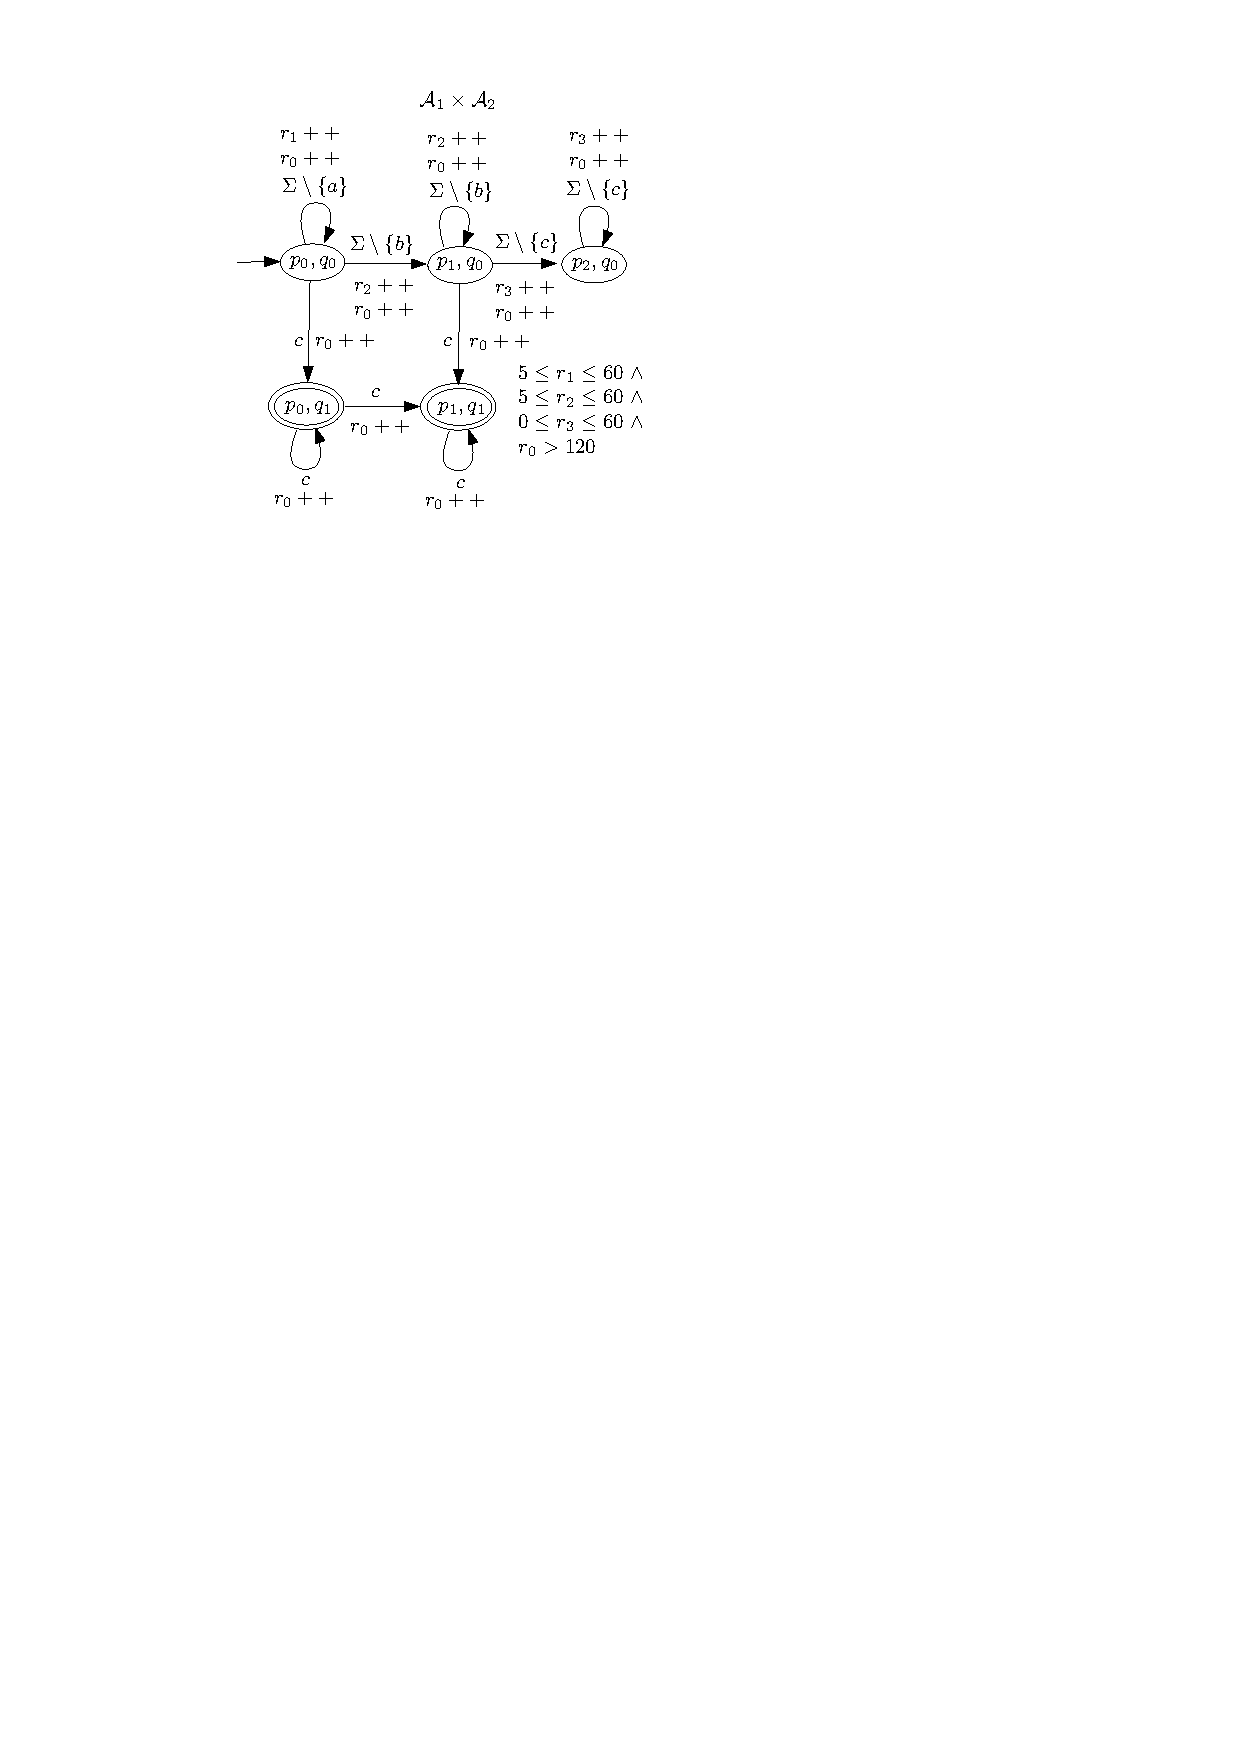
\includegraphics[width = 0.3\textwidth]{sections/overview-cefa-reduced.pdf}
  \caption{Reduced automaton $\cC$}
  \label{fig:overview:product:reduced}
\end{figure}
Furthermore, we can reduce the number of registers by merging several registers into one, if they are updated with the same value in every transition of $\aut_1 \times \aut_2$. 

At last, for the string constraints that are satisfied by a collection of strings whose lengths are small, computing LIA formulas from CEFA and solving them by SMT solvers are still expensive.  
Therefore, we introduce a heuristic of searching for solutions based on \emph{under approximations}, before computing LIA formulas and solving them by SMT solvers. More precisely, we enforce a constant upper bound $B$ on the lengths of strings and search for a $B$-bounded satisfiable assignment, that is, a satisfiable assignment where the lengths of strings are bound by $B$. Initially we set $B$ to $1$. If there does not exist a $B$-bounded satisfiable assignment, then we let $B:=B+1$ and continue the search, until finding a satisfiable assignment or reaching a given time limit. For instance, if we remove $|x| > 120$ from the string constraint~(\ref{eqn-running}), then the resulting constraint is satisfiable. Setting the bound $B$ to $1$ is already sufficient to find a solution for $\aut_1 \times \aut_2$ (with $r_0 > 120$ ignored).  





%%%%%%%%%%%%%%%%%original texts by Denghang%%%%%%%%%%%%%%%
%%%%%%%%%%%%%%%%%original texts by Denghang%%%%%%%%%%%%%%%
\hide{
\begin{figure}[ht]
  \centering
  \import{figures}{overview_example.tex}
  \caption{The CEFA handling the difficult string constraints}
  \label{fig:overview:orgin}
\end{figure}


Recalling the string constraint listed in Section \ref{sec:intro}, DPLL(T)- and automata- based string solvers can not solve it. For DPLL(T)-based string solvers, the unsatisfiability is hard to discover since it is highly related to the length and the counting, which independent derivation rules for regex and length can not conclude. For automata-based string solvers, the counting operators result in the big-size automaton, whose length abstraction is too complex to solve. To address these issues, we use automaton to encode the semantics of the counting operator, but in a smarter way by storing counting information to registers rather than unwinding it directly. The automaton model we used is called cost-enriched finite automaton(abbreviated as regex). It is carefully discussed in Section \ref{subsec:cefa}, so we briefly introduce it in this section. A CEFA can be seen as an extension of an NFA by appending symbolic updates of integers on each transition, linear integer arithmetic to constrain the integer values on each accepting state, and registers to store integer values. The main idea is based on the observation that the occurrences of exact transitions can trace the counting times, and the length can be seen as the sum of occurrences of all transitions in the accepting run. For example, the counting times in $(\Sigma \setminus a)^{\{5, 60\}}$ can be traced by the occurrences of transitions in sub-regex $\Sigma \setminus a$. To detail, we use one register to store counting, and symbolically add 1 when running one of the transitions in $\Sigma \setminus a$, tracing the counting times. Similarly, we use another register to store the length and symbolically add 1 to it when running any transition. The automaton model of string constraints \ref{eqn-running} is illustrated in Figure \ref{fig:overview}. Register $r_1$ stores the counting times of the sub-regex $\Sigma \setminus a$, register $r_2$ stores the counting times of the sub-regex $\Sigma \setminus b$, register $r_3$ stores the counting times of the sub-regex $\Sigma \setminus c$, and register $r_4$ stores the length of the string. The label $\Sigma \setminus a:(1,0,0,1)$ means that when running the transition, the counting times of $\Sigma \setminus a$ (i.e., the value of $r_1$) plus 1, and the length (i.e., the value of $r_4$) plus 1. The accepting state $q_3$ is accepting by the linear integer arithmetic $5\leq r_1\leq 60\wedge 5\leq r_2\leq 60\wedge 0\leq r_3\leq 60\wedge 120 < r_4$. $5\leq r_1\leq 40$ ensure the counting times of $\Sigma \setminus a$ is in the range $[5, 60]$, $5\leq r_2\leq 60$ ensure the counting times of $\Sigma \setminus b$ is in the range $[5, 60]$, $0\leq r_3\leq 60$ ensure the counting times of $\Sigma \setminus c$ is in the range $[0, 60]$, and $120 < r_4$ ensure the length of the string is greater than $120$. The satisfiability of the CEFA can then be reduced to the satisfiability of linear integer arithmetic, which other off-the-shelf SMT solvers solve. \newline
However, even when we use CEFA to encode counting in the string constraints, the linear integer arithmetic reduced from the CEFA still needs to be simplified to solve. The reason is that the linear integer arithmetic is solved in exponential time of the number of variables, which is linear to the sum of transitions number and states number in the CEFA. To address this issue, we use symbolic-aware simplification to reduce the number of transitions and states in the CEFA. Simply illustrating our idea, consider a simple NFA rather than a CEFA. We assume the NFA consisted of three states $q_1, q_2, q_3$, where $q_1$ is the initial state, $q_2$ and $q_3$ are the accepting states. Assume we have three transitions from $q_1$ to $q_2$ with different characters, and three transitions from $q_1$ to $q_3$. Actually, we only need to attempt some of the six transitions to get the reachable result. We run any of the transitions, and the reachability is known. So this NFA can be simplified to two states $q_1', q_2'$ where $q_1'$ is the initial state, $q_2'$ is the accepting state, and one transition from $q_1'$ to $q_2'$ with abbreviated character. The size of NFA is sharply reduced. The simplification can be done by treating the character on each transition as the same character, then applying the minimization algorithm to the NFA. CEFA can be simplified similarly, except we need to consider the counting information, i.e., symbolic updates, on each transition. For example, $a:(1)$ and $b:(1)$ are treated as the same label but $a:(1)$ and $b:(0)$ are not. Then we can apply the minimization algorithm as NFA. Recalling the CEFA (Fig. \ref{fig:overview:orgin}) handling the string constraints \ref{eqn-running}, its transitions number between $q_1$ and $q_2$ are decided by the size of alphabet $\Sigma$. We apply symbolic-aware simplification on it, then a much smaller CEFA (Fig. \ref{fig:overview:simplified}) is obtained, whose alphabet is unary so that the number of the transition between $q_1$ and $q_2$ decreases to $1$. The state number does not decrease because these three states are not mutually equivalent. 

Sometimes the string constraints are satisfiable, and the strings in the solution have a short length. Such a solution may be quickly explored by derivation rules in DPLL(T)-based string solvers but slowly explored by our approach. To improve efficiency on satisfiable string constraints, we propose a light-way heuristic that tries to find a solution in the under-approximation of the string constraints. The main idea is to explore paths within an exact length and manually compute the registers' values, rather than reduce CEFA to heavy linear integer arithmetic. For example, consider the string constraints $x \in (\Sigma \setminus a)^{\{5, 60\}} (\Sigma \setminus b)^{\{5, 60\}} (\Sigma \setminus c)^{\{0, 60\}} \wedge x \in \Sigma^* c$, we can explore paths within length 10 and get a satisfiable solution $x = cccccccccc$. 
\begin{figure}[ht]
  \centering
  \import{figures}{overview_example.tex}
  \caption{The CEFA handling the difficult string constraints}
  \label{fig:overview:orgin}
\end{figure}
\begin{figure}[ht]
  \centering
  \import{figures}{overview_example_simplified.tex}
  \caption{The simplified CEFA handling the difficult string constraints}
  \label{fig:overview:simplified}
\end{figure}
}
%%%%%%%%%%%%%%%%%original texts by Denghang%%%%%%%%%%%%%%%
%%%%%%%%%%%%%%%%%original texts by Denghang%%%%%%%%%%%%%%%

% The main idea is to use CEFAs (see Subsection \ref{subsec:cefa}) to simulate the semantics of length operations and regular memberships with bounded repetitions. As mentioned, the ESL formula contains regular literals and linear literals. The regular literal $x\in \regex$ directly results in one CEFA recognizing it (see Subsection \ref{subsec:regex2cefa}). The linear literals $\alpha_1 \leq \alpha_2$ with no length operation remain unchanged. For each linear literal $\alpha_1 \leq \alpha_2$ with length operation $|x|$, we generate a fresh variable $i$ to replace all occurrences of $|x|$ and propagate new formula $i=|x|$. Then we generate the pre-image $\aut_{i}$ whose accepting words are strings with length $i$ (see Example \ref{eg:pre_len}). After the process above, the satisfiability problem of string constraints becomes an $SAT_{CL}$ problem, which has a decision procedure to check (see Subsection \ref{subsec:emptiness}). Example \ref{example:overview} illustrate it. \newline
% \begin{example} \label{example:overview}
%   \begin{align*}
%     \varphi\equiv x\in (ab)\{1,100\}\wedge y\in ab\wedge |x| > |y|
%   \end{align*}
%   ESL conjunction $\varphi$ is made up of regular literals $x\in (ab)\{1,100\}$ and $y\in ab$, linear literals $|x| > |y|$. The linear literal is translated to $i = |x|\wedge j = |y| \wedge i > j$. Our algorithm solves the formula in four steps. First, we construct CEFAs for regular memberships $x\in (ab)\{1,100\}$ and $y\in ab$ (Fig.\ref{subfig:aut_ab1-100} and Fig.\ref{subfig:aut_ab}). Second, we compute the pre-images of length operations $i=|x|$ and $j=|y|$ (Fig.\ref{subfig:preimage_x} and Fig.\ref{subfig:preimage_y}). Then we intersect pre-images to automata corresponding to the regular memberships for each string variable (Fig.\ref{subfig:aut_x} and Fig.\ref{subfig:aut_y}). We translate the satisfiability problem of $\varphi$ to the emptiness checking problem of automata (Fig.\ref{subfig:preimage_x} and Fig.\ref{subfig:preimage_y}) under linear arithmetic constants $i > y$, which could be solved by the decision procedure illustrated in section \ref{sec:algorithm}.

  % \begin{figure}[h]
  %   \begin{subfigure}[b]{0.49\textwidth}
  %     \centering
  %     \begin{tikzpicture}[
  %       shorten >=1pt,node distance=2cm,on grid,>={Stealth[round]},
  %       initial text=, every state/.style={minimum size = 0.001cm},
  %       accepting text=$1\leq r_1\leq 100$, accepting/.style=accepting by arrow,
  %       accepting where=above
  %       ]

  %       \node[state,initial]            (q_0)                      {};
  %       \node[state]                    (q_1) [right=of q_0]       {};
  %       \node[state,accepting]          (q_2) [right=of q_1]       {};

  %       \path[->] (q_0) edge              node      [above]           {$a$/(1)} (q_1)
  %       (q_1) edge              node      [above]           {$b$/(0)} (q_2)
  %       (q_2) edge [bend left]  node      [below]           {$a$/(1)} (q_1);
  %     \end{tikzpicture}
  %     \caption{The CEFA recognizing $(ab)\{1,100\}$}
  %     \label{subfig:aut_ab1-100}
  %   \end{subfigure}
  %   \begin{subfigure}[b]{0.49\textwidth}
  %     \centering
  %     \begin{tikzpicture}[
  %       shorten >=1pt,node distance=2cm,on grid,>={Stealth[round]},
  %       initial text=, every state/.style={minimum size = 0.001cm},
  %       accepting text=$\top$, accepting/.style=accepting by arrow,
  %       accepting where=above
  %       ]

  %       \node[state,initial]            (q_0)                      {};
  %       \node[state]                    (q_1) [right=of q_0]       {};
  %       \node[state, accepting]         (q_2) [right=of q_1]       {};

  %       \path[->] (q_0) edge              node      [above]           {$a$/()} (q_1)
  %       (q_1) edge              node      [above]           {$b$/()} (q_2);
  %     \end{tikzpicture}
  %     \caption{The CEFA recognizing $ab$}
  %     \label{subfig:aut_ab}
  %   \end{subfigure}
  %   \begin{subfigure}[b]{0.49\textwidth}
  %     \centering
  %     \begin{tikzpicture}[
  %       shorten >=1pt,node distance=2cm,on grid,>={Stealth[round]},
  %       initial text=, every state/.style={minimum size = 0.001cm},
  %       accepting text=${r_2 = i}$, accepting/.style=accepting by arrow,
  %       ]

  %       \node[state,initial,accepting]            (q_0)       {};

  %       \path[->] (q_0) edge [loop below] node{$\Sigma$/(1)} ();
  %     \end{tikzpicture}
  %     \caption{The pre-image of $i = |x|$}
  %     \label{subfig:preimage_x}
  %   \end{subfigure}
  %   \begin{subfigure}[b]{0.49\textwidth}
  %     \centering
  %     \begin{tikzpicture}[
  %       shorten >=1pt,node distance=2cm,on grid,>={Stealth[round]},
  %       initial text=, every state/.style={minimum size = 0.001cm},
  %       accepting text=${r_3 = j}$, accepting/.style=accepting by arrow,
  %       ]

  %       \node[state,initial,accepting]            (q_0)       {};

  %       \path[->] (q_0) edge [loop below] node{$\Sigma$/(1)} (1);
  %     \end{tikzpicture}
  %     \caption{The pre-image of $j = |y|$}
  %     \label{subfig:preimage_y}
  %   \end{subfigure}
  %   \begin{subfigure}[b]{0.49\textwidth}
  %     \centering
  %     \begin{tikzpicture}[
  %       shorten >=1pt,node distance=2cm,on grid,>={Stealth[round]},
  %       initial text=, every state/.style={minimum size = 0.001cm},
  %       accepting text=${r_2 = i\wedge 1\leq r_1 \leq 100}$, accepting/.style=accepting by arrow,
  %       accepting where=above
  %       ]

  %       \node[state,initial]            (q_0)                      {};
  %       \node[state]                    (q_1) [right=of q_0]       {};
  %       \node[state,accepting]          (q_2) [right=of q_1]       {};

  %       \path[->] (q_0) edge node [above]  {$a$/(1,1)} (q_1)
  %       (q_1) edge           node [above]  {$b$/(0,1)} (q_2)
  %       (q_2) edge [bend left]  node      [below]           {$a$/(1,1)} (q_1);
  %     \end{tikzpicture}
  %     \caption{The final automaton of $x$}
  %     \label{subfig:aut_x}
  %   \end{subfigure}
  %   \begin{subfigure}[b]{0.49\textwidth}
  %     \centering
  %     \begin{tikzpicture}[
  %       shorten >=1pt,node distance=2cm,on grid,>={Stealth[round]},
  %       initial text=, every state/.style={minimum size = 0.001cm},
  %       accepting text=${r_3=j}$, accepting/.style=accepting by arrow,
  %       accepting where=above
  %       ]

  %       \node[state,initial]            (q_0)                      {};
  %       \node[state]                    (q_1) [right=of q_0]       {};
  %       \node[state, accepting]         (q_2) [right=of q_1]       {};

  %       \path[->] (q_0) edge    node      [above]           {$a$/(1)} (q_1)
  %       (q_1) edge              node      [above]           {$b$/(1)} (q_2);
  %     \end{tikzpicture}
  %     \caption{The final automaton of $y$}
  %     \label{subfig:aut_y}
  %   \end{subfigure}
  %   \caption{All automata used in the example \ref{example:overview}}
  % \end{figure}


% \end{example}

% \pagebreak
